\documentclass[
  captions=tableheading,
  bibliography=totoc, 
  titepage=firstiscover,
]{scrartcl}

\usepackage{blindtext} %neuer input

\usepackage{longtable} % Tabellen über mehrere Seiten

\usepackage[utf8]{inputenc} %neuer input

\usepackage{scrhack}

\usepackage[aux]{rerunfilecheck} %Warnung falls nochmal kompiliert werden muss

\usepackage{fontspec} %Fonteinstellungen

\recalctypearea{}

\usepackage[main=ngerman]{babel} %deutsche Spracheinstellung

\usepackage{ragged2e} %neuer input

\usepackage{amsmath, nccmath}

\usepackage{amssymb} %viele mathe Symbole

\usepackage{mathtools} %Erweiterungen für amsmath


\DeclarePairedDelimiter{\abs}{\lvert}{\rvert}
\DeclarePairedDelimiter{\norm}{\lVert}{\rVert}

\DeclarePairedDelimiter{\bra}{\langle}{\rvert}
\DeclarePairedDelimiter{\ket}{\lvert}{\rangle}

\DeclarePairedDelimiterX{\braket}[2]{\langle}{\rangle}{
#1 \delimsize| #2
}

\NewDocumentCommand \dif {m}
{
\mathinner{\symup{d} #1}
}


\usepackage[
  math-style=ISO,
  bold-style=ISO,
  sans-style=italic,
  nabla=upright,
  partial=upright,
  warnings-off={
    mathtools-colon,
    mathtools-overbracket,
  },
]{unicode-math}

\setmathfont{Latin Modern Math}
\setmathfont{XITS Math}[range={scr, bfscr}]
\setmathfont{XITS Math}[range={cal, bfcal}, StylisticSet=1]


\usepackage[
  locale=DE,
  separate-uncertainty=true,
  per-mode=reciprocal,
  output-decimal-marker={,},
]{siunitx}

\usepackage[autostyle]{csquotes} %richtige Anführungszeichen

\usepackage{xfrac}

\usepackage{float}

\floatplacement{figure}{htbp}

\floatplacement{table}{htbp}

\usepackage[ %floats innerhalb einer section halten
  section,   %floats innerhalb er section halten
  below,     %unterhalb der Section aber auf der selben Seite ist ok
]{placeins}

\usepackage[
  labelfont=bf,
  font=small,
  width=0.9\textwidth,
]{caption}

\usepackage{subcaption} %subfigure, subtable, subref

\usepackage{graphicx}

\usepackage{grffile}

\usepackage{booktabs}

\usepackage{microtype} %Verbesserungen am Schriftbild

\usepackage[
backend=biber,
]{biblatex}

\addbibresource{../lit.bib}

\usepackage[ %Hyperlinks im Dokument
  german,
  unicode,
  pdfusetitle,
  pdfcreator={},
  pdfproducer={},
]{hyperref}

\usepackage{bookmark}

\usepackage[shortcuts]{extdash}

%\usepackage{warpcol}


\begin{document}
    \title{V702 Aktivierung mit Neutronen }
    \author{  
    Tobias Rücker\\
    \texorpdfstring{\href{mailto:tobias.ruecker@tu-dortmund.de}{tobias.ruecker@tu-dortmund.de}
    \and}{,} 
    Paul Störbrock\\
    \texorpdfstring{\href{mailto:paul.stoerbrock@tu-dortmund.de}{paul.stoerbrock@tu-dortmund.de}}{}
    }
    \date{Durchführung: 26.05.2020, Abgabe: 02.06.20 \vspace{-4ex}}
\maketitle
\thispagestyle{empty}

\newpage
\tableofcontents
\thispagestyle{empty}
\newpage

% Ziel %%%%%%%%%%%%%%%%%%%%%%%%%%%%%%%%%%%%%%%%%%%%%%%%%%%%%%%%%%%%%%%%%%%%%%%%%%%%%%%%%%%%%%%%%%%%%%%%%%%%%%%%%%%%%%%%%%%%%%%%%%%%%%%%%%%%%%%%%%%%%%%%%%%%%%%%%%%%%%%%%%%%%%%%%%%%%%%%%%%%%%%%%%%%%%%%%%%%%%%%%%%%%%%%%

\setcounter{page}{1}
\section{Ziel}\justifying
Die Kenntnis über die Stabilität von Atomen und den Verlaufsprozess von verschiedenen
Zerfällen spielt nicht nur bei Messungen in der Physik, sondern vor allem auch in der 
Medizin zum Beispiel in der Krebsbehandlung eine Rolle. Daher wird im Folgenden die Halbwertszeit von
zwei Materialien bestimmt, indem diese mit energiearmen Neutronen beschossen werden und die Teilchen mittels 
einem Geiger-Müller-Zählrohr gezählt werden.

% Theorie %%%%%%%%%%%%%%%%%%%%%%%%%%%%%%%%%%%%%%%%%%%%%%%%%%%%%%%%%%%%%%%%%%%%%%%%%%%%%%%%%%%%%%%%%%%%%%%%%%%%%%%%%%%%%%%%%%%%%%%%%%%%%%%%%%%%%%%%%%%%%%%%%%%%%%%%%%%%%%%%%%%%%%%%%%%%%%%%%%%%%%%%%%%%%%%%%%

\section{Theorie}\justifying
Die Stabilität von Atomen hängt stark von dem Verhältnis der Protonen und Neutronen ab. Sind
Atome nicht stabil, zerfallen sie zu stabile oder instabile Kernen, wo bei instabilen der Zerfallsprozess
noch nicht beendet ist.  Eine wichtige Eigenschaft des Zerfallsprozesses stellt die Halbwertszeit T
dar. Sie beschreibt die Zeit, nach der die Hälfte der Kerne einer Menge zerfallen sind.
Für die Messung der Halbwertszeit in einer Größenordnung von Stunden und Sekunden werden
stabile Kerne mit Neutronen beschossen. Diese Kerne werden nach der Absorption des Neutrons zu einem Zwischenkern $A^*$, welcher
auch Compoundkern genannt wird. Die Energie des Neutrons verteilt sich auf die anderen Nukleonen,
wodurch diese in höhere Energiezustände gebracht werden. Bei Neutronen mit geringen 
Energien kann kein Nukleon abgestoßen werden, weshalb es unter Aussendung eines Gammaquants in den Grundzustand übergeht \cite{V702}
\begin{align}
    \ce{_z^mA + _0^1n -> _z^{m+1}A^* -> _z^{m+1} A + \symup{\gamma}}. \label{eq:1} %hier steht das erste plus im exponenten
\end{align}
Dabei gibt m die Massenzahl, z die Ordnungszahl, n das eingesendete Neutron, A den beschossenen Kern,
$A^*$ den Zwischenkern und $\gamma$ den ausgesendeten Gammaquant an. Durch das zusätzliche
Neutron ist der Kern nun instabil und zerfällt \cite{V702}
\begin{align}
    \ce{_z^{m+1}A -> _{z+1}^{m+1}C + \symup{\beta}^- + E_{\text{kin}} + \bar{\symup{\nu}}_e } \label{eq:2}.
\end{align}
Hierbei ist C der aus dem Zerfall entstehende Kern, $\beta ^-$ ein Elektron und $\bar{\nu}_e$ ein Elektron-Antineutrino.
Die Masse der Teilchen auf der linken Seite der Reaktionsgleichung ist größer als die der Teilchen auf
der rechten Seite. Diese Energie geht in Form von kinetischer Energie an das Elektron und
Elektron-Antineutrino. Um möglichst viele Zerfälle für eine Messung zu erzeugen wird ein
entsprechend hoher Wirkungsquerschnitt $\sigma$ benötigt. Der Wirkungsquerschnitt beschreibt
die Fläche, die der Atomkern haben müsste, damit jedes Neutron mit der Fläche wechselwirkt.
Für eine geringe Energie der Neutronen gegenüber des Zwischenkerns ergibt sich folgende
Proportionalität für den Wirkungsquerschnitt \cite{V702}
\begin{align}
    \sigma \sim \frac{1}{v}, \label{eq:3}
\end{align}
wobei v die Geschwindigkeit der Neutronen ist.
Aufgrund der Proporionalität sind niederenergetische Neutronen für die Messung notwendig,
was verständlich ist, da eine kleinere Energie eine geringere Geschwindigkeit bedeutet
und sich das Neutron dadurch länger in der Einwirkssphähre befindet.\\
Für die Erzeugung von Neutronen kann die Reaktion von Beryllium mit 
Alpha-Teilchen genutzt werden \cite{V702}
\begin{align}
    \ce{ ^9 Be + _2^4 \symup{\alpha} -> _6^{12} C + _0^1n }. \label{eq:4}
\end{align}
Die $\alpha$-Teilchen entstehen dabei aus dem Zerfall von $^{226} $Ra-Kerne.
Da die Neutronen nach der Reaktion noch zu energiereich sind, wird eine dicke Materieschicht (Abb. \ref{fig:1}, Nr. 2) eingebracht,
durch die die Neutronen hindurchdiffundieren müssen. Die Kerne davon sollten auf
einer gleichen Größenordnung wie die Neutronen sein, damit der Energieübertrag am größten ist.
Daher eignet sich Paraffin dafür. Ein schematischer Aufbau für so eine Quelle ist in der folgenden Abbildung
dargestellt:
\begin{figure}[H]
    \centering
    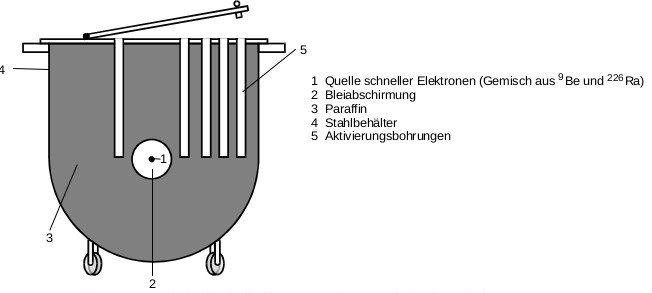
\includegraphics[width=\linewidth]{images/neutron_quelle.jpg}
    \caption{Schematischer Aufbau einer Neutronenquelle \cite{V702}.
    Durch den Zerfall von Radium-Kernen entstehen $\alpha$-Teilchen,
    welche mit den Beryllium-Atomen wechselwirken. Dadurch entstehen Neutronen,
    welche im Paraffin einen Teil ihrer Energie abgeben und damit abgebremst werden.
    }
    \label{fig:1}
\end{figure}
Die abgebremsten Neutronen haben eine kinetische Energie, welche der mittleren Energie der Umgebung entspricht und
werden thermische Neutronen genannt.\\
Für Messungen wird eine zylindrische Probe in einen Aktivierungsschacht gebracht.
Da es schwer ist die Zerfallsrate pro Zeit genau zu bestimmen, wird die Anzahl der 
Zerfälle über ein Zeitintervall $\Delta t$ betrachtet. Dafür ergibt sich ein
einfacher exponentieller Zusammenhang \cite{V702}
\begin{align}
    N_{\Delta t} (t) = N_0 (1-e^{\lambda \Delta t}) e^{- \lambda t}. \label{eq:5} 
\end{align}
Dabei stellt $N_0$ die zu Messbeginn vorhandene Anzahl an instabilen Kernen und $\lambda$ die Zerfallskonstante dar.
Die Halbwertszeit lässt sich über die Formel \cite{V702}
\begin{align}
    T=\frac{\ln(2)}{\lambda} \label{eq:6}
\end{align}
berechnen.\\
Eine geeignete Wahl des Zeitintervalls ist wichtig, da es ansonsten zu hohen
statistischen oder systematischen Fehlern kommt.\\
Manche Materialien wie Rhodium haben zwei Zerfallsketten\\
$\ce{^{103}_{45}Rh + n}  
\begin{cases}
    \ce{\stackrel{10\%}{\to} ^{104i}_{45}Rh +\symup{\gamma} -> ^{104}_{46}Pd+\symup{\beta}^- + \bar{\symup{\nu}}_e }\\
    \ce{\stackrel{90\%}{\to} ^{104}_{45}Rh ->  ^{104}_{46}Pd+\symup{\beta}^- + \bar{\symup{\nu}}_e }
\end{cases}.\text{\cite{V702}}
$
Das i beim Rhodium steht für einen isomeren Kern, welcher sich nur in der Energie und
Halbwertszeit vom Rhodium-Kern unterscheidet.\\
Da der isomere Kern kurzlebiger ist, wird ab einem gewissen Zeitpunkt $t^*$ hauptsächlich
die andere Zerfallskette gemessen, was sich in der folgenden Abbildung zu erkennen ist:
\begin{figure}[H]
    \centering
    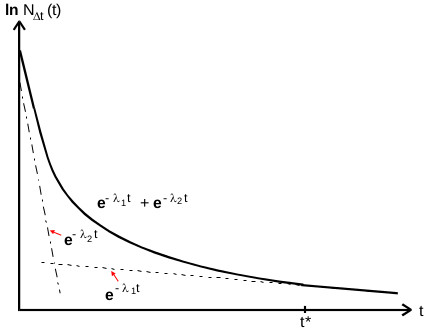
\includegraphics[width=\linewidth]{images/Rh_theo.jpg}
    \caption{Logarithmische Darstellung eines zeitlichen Zerfalls mit
    2 Zerfallsketten \cite{V702}.
    Die gestrichelten Linien zeigen den potentiellen Verlauf der Geraden für die 
    einzelnen Komponenten der Zerfallsreaktion. Der Zeitpunkt $t^*$ markiert den Übergang, ab
    dem der kurzlebigere Kern kaum noch einen Einfluss hat und eine Gerade entsteht.
    }
    \label{fig:2}
\end{figure}


% Versuchsaufbau + Versuchsdurchführung %%%%%%%%%%%%%%%%%%%%%%%%%%%%%%%%%%%%%%%%%%%%%%%%%%%%%%%%%%%%%%%%%%%%%%%%%%%%%%%%%%%%%%%%%%%%%%%%%%%%%%%%%%%%%%%%%%%%%%%%%%%%%%%%%%%%%%%%%%%%%%%%%%%%%%%%%%%%%%%%%%%%%%%%%%%%%%%%%%%%%%%%%%%%%%%%%%

\section{Versuchsaufbau und Versuchsdurchführung}\justifying

% Auswertung %%%%%%%%%%%%%%%%%%%%%%%%%%%%%%%%%%%%%%%%%%%%%%%%%%%%%%%%%%%%%%%%%%%%%%%%%%%%%%%%%%%%%%%%%%%%%%%%%%%%%%%%%%%%%%%%%%%%%%%%%%%%%%%%%%%%%%%%%%%%%%%%%%%%%%%%%%%%%%%%%%%%%%%%%%%%%%%%%%%%%%%%%%%%%%%%%%

\section{Auswertung}

\subsection{Vanadium}% Provisorische Namen!

\begin{figure}
    \centering
    \includegraphics[width=\linewidth]{build/plot_V.pdf}
    \caption{} % Caption noch hinzufügen
    \label{fig:a} % Ändern  sobald Reihenfolge feststeht
\end{figure}

\subsection{Rhodium} % Provisorische Namen!

\begin{figure}
    \centering
    \includegraphics[width=\linewidth]{build/plot_Rh.pdf}
    \caption{} % Caption noch hinzufügen
    \label{fig:b} % Ändern  sobald Reihenfolge feststeht
\end{figure}

% Diskussion %%%%%%%%%%%%%%%%%%%%%%%%%%%%%%%%%%%%%%%%%%%%%%%%%%%%%%%%%%%%%%%%%%%%%%%%%%%%%%%%%%%%%%%%%%%%%%%%%%%%%%%%%%%%%%%%%%%%%%%%%%%%%%%%%%%%%%%%%%%%%%%%%%%%%%%%%%%%%%%%%%%%%%%%%%%%%%%%%%%%%%%%%%%%%%%%%%

\section{Diskussion}


% Literatur %%%%%%%%%%%%%%%%%%%%%%%%%%%%%%%%%%%%%%%%%%%%%%%%%%%%%%%%%%%%%%%%%%%%%%%%%%%%%%%%%%%%%%%%%%%%%%%%%%%%%%%%%%%%%%%%%%%%%%%%%%%%%%%%%%%%%%%%%%%%%%%%%%%%%%%%%%%%%%%%%%%%%%%%%%%%%%%%%%%%%%%%%%%%%%%%%%

\newpage
\printbibliography

\end{document}